% Path diagram of the vector autoregressive model (vignette var).
\documentclass[tikz, border = 6pt]{standalone}
\usepackage{amsmath}
\usepackage{bm}
\usetikzlibrary{arrows.meta, positioning, calc}
\tikzset{
  lat/.style = {circle, draw, thick, minimum size = 12mm, inner sep = 0pt},
  obs/.style = {rectangle, draw, thick, minimum size = 10mm, inner sep = 1pt},
  noise/.style = {circle, draw, minimum size = 7mm, inner sep = 0pt},
  reg/.style = {-{Stealth[length = 2.5mm]}, thick},
  cov/.style = {{Stealth[length = 2mm]}-{Stealth[length = 2mm]}},
  lab/.style = {font = \footnotesize, fill = white, inner sep = 1pt},
  dots/.style = {font = \Large}
}
\begin{document}
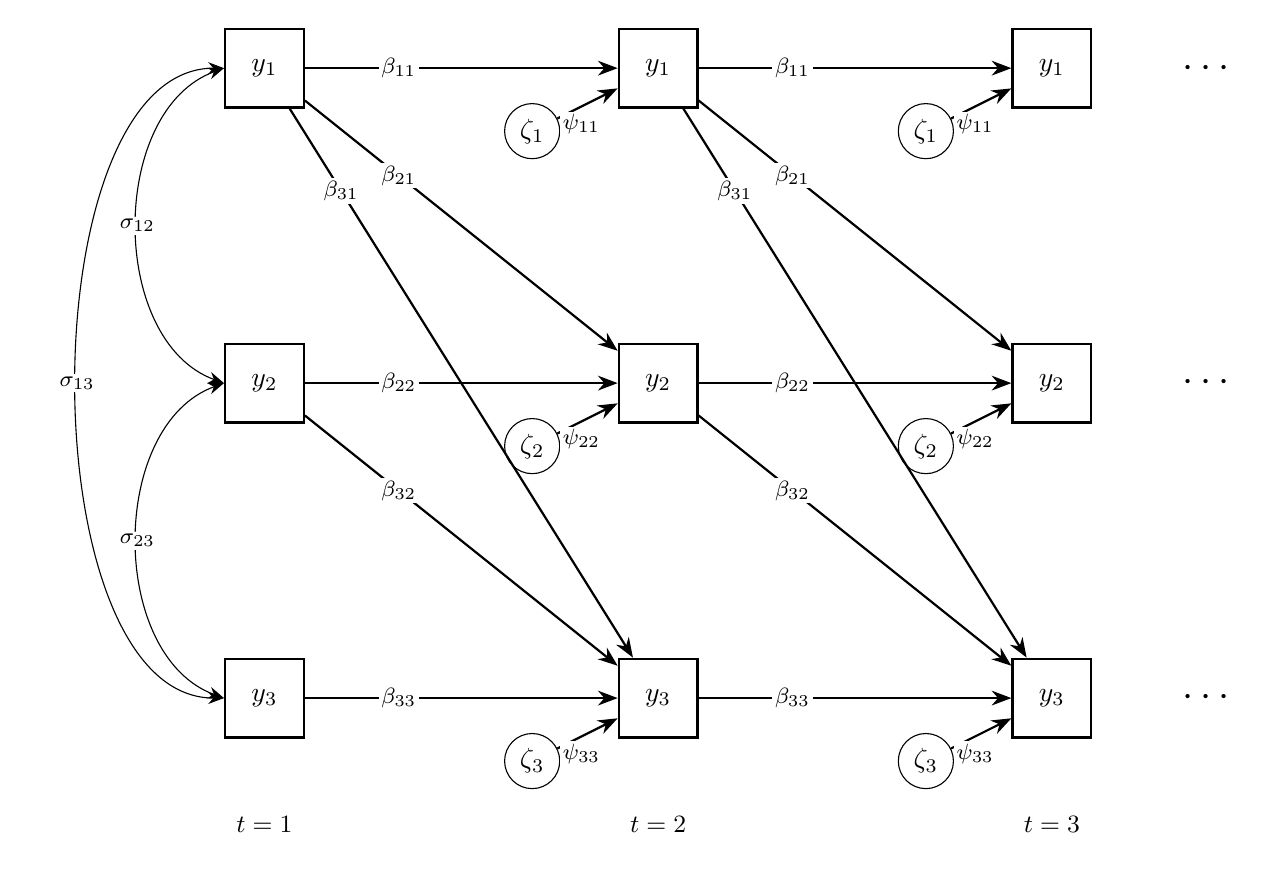
\begin{tikzpicture}
  \foreach \t/\x in {1/0, 2/5, 3/10} {
    \foreach \jj/\rr in {1/0, 2/-4, 3/-8} {
      \node[obs] (e\jj\t) at (\x, \rr) {$y_{\jj}$};
    }
    \node[font = \small] at (\x, -9.6) {$t = \t$};
  }
  % dynamics
  \foreach \s/\t in {1/2, 2/3} {
    \foreach \jj in {1, 2, 3} {
      \draw[reg] (e\jj\s) -- node[lab, pos = 0.3] {$\beta_{\jj\jj}$} (e\jj\t);
    }
    \draw[reg] (e1\s) -- node[lab, pos = 0.3] {$\beta_{21}$} (e2\t);
    \draw[reg] (e1\s) -- node[lab, pos = 0.15] {$\beta_{31}$} (e3\t);
    \draw[reg] (e2\s) -- node[lab, pos = 0.3] {$\beta_{32}$} (e3\t);
  }
  % process noise
  \foreach \t/\x in {2/5, 3/10} {
    \foreach \jj/\rr in {1/0, 2/-4, 3/-8} {
      \node[noise] (z\jj\t) at (\x - 1.6, \rr - 0.8) {$\zeta_{\jj}$};
      \draw[reg] (z\jj\t) -- node[lab, pos = 0.4, below = 0.5mm] {$\psi_{\jj\jj}$} (e\jj\t);
    }
  }
  % initial condition
  \draw[cov] (e11.west) to[out = 200, in = 160] node[lab] {$\sigma_{12}$} (e21.west);
  \draw[cov] (e21.west) to[out = 200, in = 160] node[lab] {$\sigma_{23}$} (e31.west);
  \draw[cov] (e11.west) .. controls (-3, 0) and (-3, -8) .. node[lab] {$\sigma_{13}$} (e31.west);
  \foreach \rr in {0, -4, -8} {
    \node[dots] at (12, \rr) {$\cdots$};
  }
\end{tikzpicture}
\end{document}
